\vspace{-1em}
\section {ECN versus Delay}
\label{sec:discuss}

We have now seen that DCQCN and TIMELY (with a small modification) perform
generally well, if properly tuned for a given scenario. Can we thus conclude
that ECN and delay are both "equivalent" signals, when it comes to congestion
control? 

We believe that the answer is no, because ECN has two potential advantages, as
discussed below.

\para{ECN marking is done on packet egress:}
Modern shared-buffer switches, especially those that use Broadcom's merchant
silicon, do ECN marking on {\em packet egress}. When a packet is ready to
depart, the controller checks the egress queue for that port {\em at that
instant}, and marks the packet according to the specified algorithm
(e.g.  Equation~\ref{eq:mark}). Thus, the mark conveys information about the
state of the queue at the time the packet {\em departure}.

RTT measurements are different: If the egress queue discipline is FIFO within a
priority class (which it typically is), the delay experienced by a packet
reflects the state of the queue at the time the packet {\em arrives} at the
queue. 

This means that the control signal carried by the ECN mark is delayed only by
the propagation delay, but the control signal carried by the RTT signal is
delayed both by the queuing delay as well as the propagation delay. 

This is a subtle difference: the claim is not that ECN carries more information;
it that the delay of the control loop is decoupled from the queuing delay.

This is why the DCQCN fluid model (Figure~\ref{fig:dcqcn_model}) assumes that
the control loop delay is constant.\footnote{DCTCP fluid model
in~\cite{dctcp-analysis} makes the same assumption.} We cannot make the same
assumption for TIMELY, and  thus we incorporate $\tau'$ and
Equation~\ref{eq:timely_taup} in the TIMELY fluid model
(Figure~\ref{fig:timely_model}).

This means that as the queue length increases (e.g. when there are
more flows), congestion control algorithms that rely on RTT suffer from
increasing {\em lag} in their control loop, making them more difficult to control. We see this
happening for TIMELY (Figure~\ref{fig:timely_stability}). DCQCN is
affected less by  this
effect (Figure~\ref{fig:dcqcn_stability_default}).

This issue has gone unnoticed in the congestion control literature so far,
because most of it has focused on wide area networks.  In wide area networks,
queuing delays and propagation delays can be comparable (excluding scenarios
like buffer bloat~\cite{bufferbloat}). However, in data center networks, queuing
delays can easily dominate switching and propagation delays.  For example, an
Arista 7050QX32 has 40Gbps ports, and a total shared buffer of switch has 12MB.
Even if just 1MB worth of queue builds up at an egress port,\footnote{This
requires enabling dynamic thresholding, but it is almost always enabled in real
deployments.} it takes 200 $\mu$s to drain it. In contrast, the one-hop
propagation delay, with cut-through forwarding, is around 1-2 $\mu$s.  Typical
DC network diameter is 6 hops, so overall propagation delay is under $25\mu s$.

The reader may argue that it is easy to fix this issue  -- all we have to do is
to build a delay-based protocol that strives to keep the  bottleneck queue
(more-or-less) constant. Then, the control signal delay experienced by the RTT
feedback signal is also fixed, albeit a little higher (propagation delay, plus
fixed queuing delay). 

However, a delay based congestion control protocol that maintains a fixed
queue, cannot ensure fairness.

\para{For delay-based control, fixed queue comes at the cost of fairness:}
One way to build protocols that guarantee delay to a fixed quantity is to use
a controller with \emph{integral} control~\cite{hollot2001designing,REM}.  The idea behind integral control
is to look at an error signal, {\em e.g.,} the difference between the actual queue
length and a desired or reference queue length, and adjust the feedback until
the error signal goes to 0. A stable PI controller is guaranteed to achieve
this. In a continuous system, the feedback signal $p(t)$ evolves in the
following way with a PI controller:
\begin{equation}
\small
\frac{dp}{dt} = K_1 \frac{de}{dt}+K_2e(t)
\end{equation}
When the feedback signal converges, both the error signal $e(t)$ as
well as the derivative of the error signal, $de/dt$ must converge to
0. The derivative of the error signal, (the derivative of the queue length), goes to 0
when the sum of the rates $R_i$ match the link capacity $C$. The error signal itself goes to 0
when the queue length matches the reference value. Thus the integral
controller implements the ``match rate, clear buffer'' scheme
presented in~\cite{REM}. 

For DCQCN we can implement the PI controller to mark the packets at the switch
instead of RED (which is a proportional controller without the integral action)
and use that $p$ in the usual way to perform the multiplicative decrease. 

For (patched) TIMELY, we can measure the delay at the end hosts and implement a
PI controller by generating an internal variable ``$p$'', using the error signal
``$e(t)$'' as the difference between the measured delay and some
desired delay. This internal variable $p$ can then replace the $\tfrac{{q(t -
\tau ') - q'}}{{q'}}$ term in Equation (\ref{eq:timely_fixed}) as the feedback
to control the rates.

We implemented the PI controller for both the DCQCN and patched TIMELY fluid
models and performed simulations. As we see in Figure~\ref{fig:dcqcn_pi}~for
DCQCN, all the flows converge to the same (fair) rate and the queue length is stabilized to a preconfigured value, regardless of
the number of flows (as well as regardless of propagation delay). This is
important not only for stability, but also for performance reasons in a data
center networks, where is important to ensure that completion times for short
flows do not suffer from excessive queuing delays~\cite{dctcp}.

\begin{figure}
\subfigure {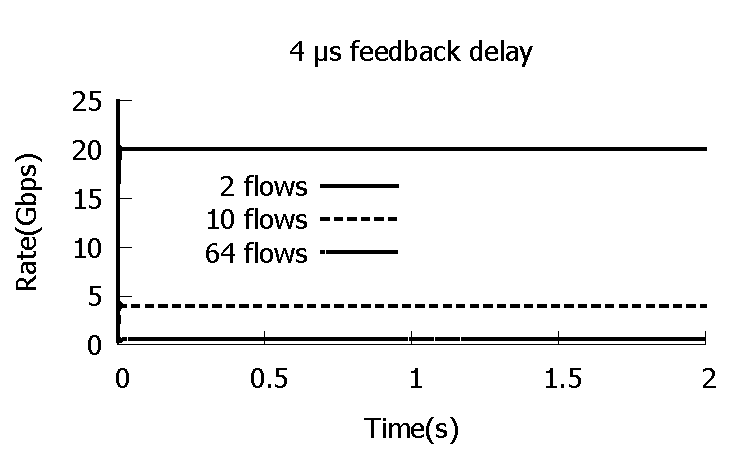
\includegraphics[width=0.49\columnwidth]{figures/stable_rate_4_pifixed.pdf}}
\subfigure {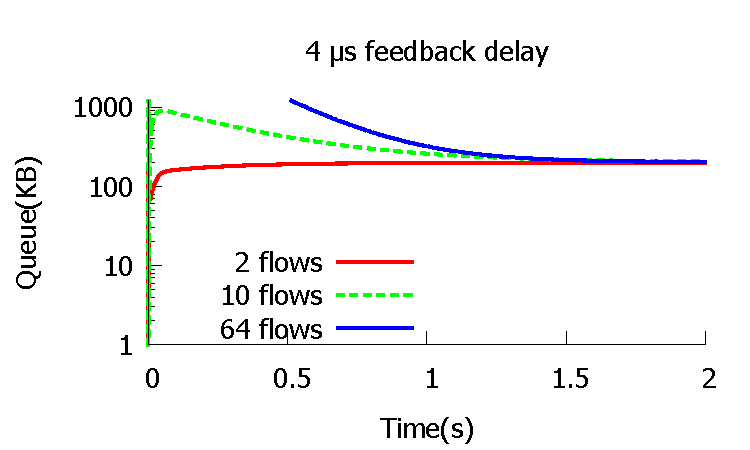
\includegraphics[width=0.49\columnwidth]{figures/stable_q_4_pifixed.pdf}}
\vspace{-1em}
\caption{DCQCN with PI controller}
\label{fig:dcqcn_pi}
\vspace{-1em}
\end{figure}

In contrast, when we use a PI controller at the end hosts with patched
TIMELY, we see that although we can control the queue
to a specified value (300 KB), we cannot achieve fairness (Figure~\ref{fig:timely_pi}). 
Thus, while patched TIMELY was able to achieve fairness without guaranteeing
delay, with PI it is able to guarantee delay without
achieving fairness.
\begin{figure}
\center
\subfigure[Two flows (7 and 3Gbps)]
{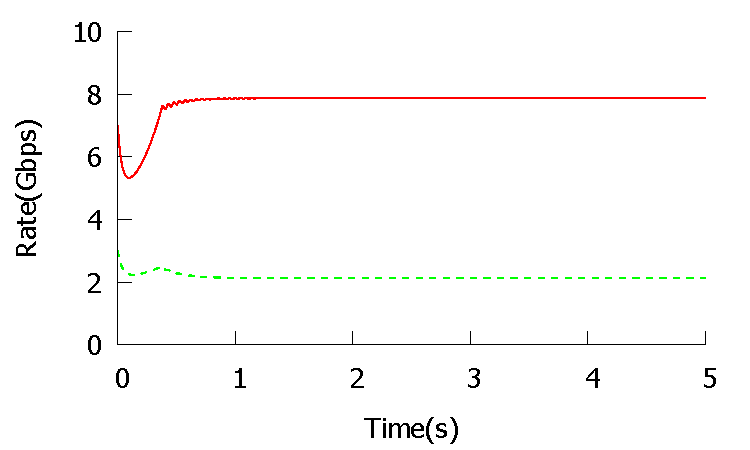
\includegraphics[width=0.49\columnwidth]{figures/timely_withpi_2_4_rate.pdf}}
\subfigure[Two flows (7 and 3Gbps)] {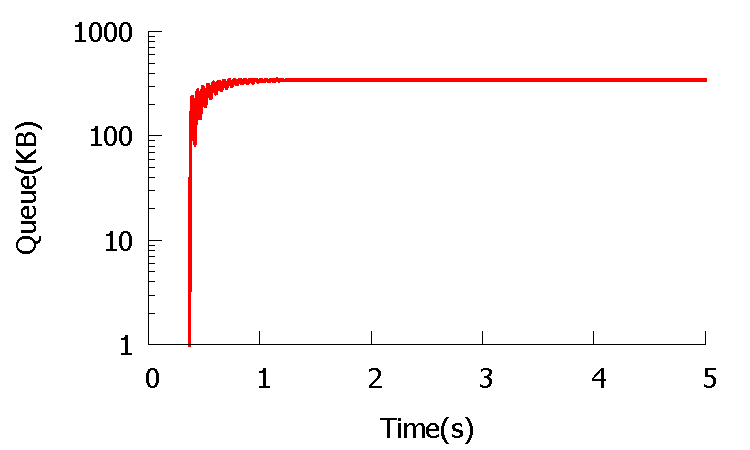
\includegraphics[width=0.49\columnwidth]{figures/timely_withpi_2_4_queue.pdf}}
\subfigure[Ten flows] {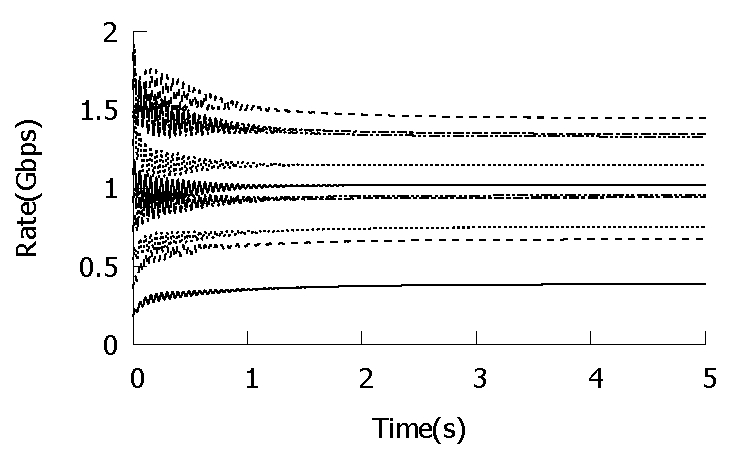
\includegraphics[width=0.49\columnwidth]{figures/timely_withpi_10_4_rate.pdf}}
\subfigure[Ten flows] {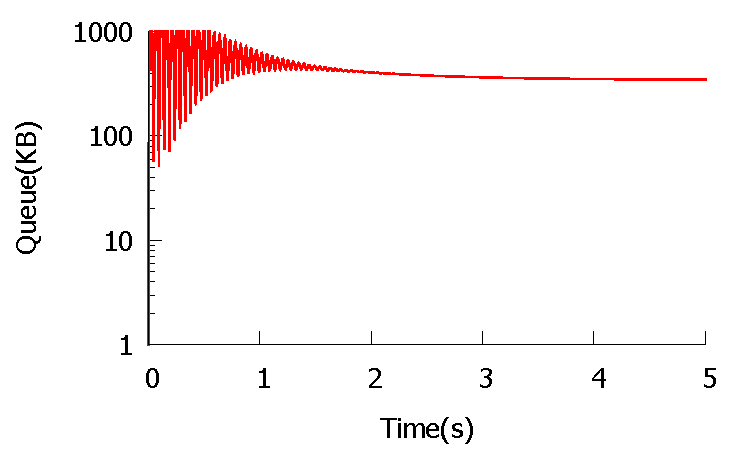
\includegraphics[width=0.49\columnwidth]{figures/timely_withpit_10_4_queue.pdf}}
\vspace{-1em}
\caption{PI controller to stabilize TIMELY}
\vspace{-1em}
\label{fig:timely_pi}
\end{figure}

We next prove a result that formalizes this fundamental tradeoff between fairness
and guaranteed delay for protocols that rely on delay measurements at the end
points to implement congestion control. We first assume that the
steady state throughput achieved by a congestion control transport
protocol is a function of the observed delay $d$ and some feedback
value $p$. The value of $p$ can be the loss probability or the ECN marking
probability or some internal variable $p$ computed by the patched
TIMELY+PI mechanism we described above. Thus,
$R = f(d,p)$ for steady state throughput $R$ and some function $f(d,p)$. Then the
following theorem formalizes the fairness/delay tradeoff in such systems.

\begin{thm}[Fairness/Delay tradeoff]
\label{thm:fairness-delay}
For congestion control mechanisms that have steady state throughput of
the kind $R = f(d,p)$, for some function $f$, delay $d$ and
feedback $p$, if the feedback is based on purely end to end
delay measurements, you can either have fairness or a fixed delay, 
but not both simultaneously.
\end{thm}
\begin{proof}
To guarantee fairness, the system must have a
unique fixed point. 
Consider $N$ flows sharing a link of capacity $C$. 
Then, for each flow, we have 
$ R_i = f(d,p_i), i = 1,\ldots,N.$
There is an additional equation constraining the throughput at the
link, $\sum R_i = C$.
Hence we have $N+1$ equations and $2 N$ unknowns -- $\{R_i,p_i\},
 i=1\ldots,N$. This is an underdetermined system with infinite (or no)
solutions. To make this system consistent, we need a common $p_i$,
reducing the number of variables to $N+1$. That can be achieved
either by marking at the switch (violating the assumption of delay
being the only feedback), or by making this $p_i$ a function of
the (common) queue length. However if we control the delay to a fixed quantity,
it becomes agnostic of the number of flows which will make the system
of equations inconsistent, since the constraint $\sum_i R_i = C$
implies the steady state throughput of a flow depends on the number of
flows contending. Thus, to make the system consistent $p_i$ has to be
a function of the common queue length which depends on the number of flows 
and hence we cannot control the delay to a fixed quantity. 
\end{proof}
Note that the preceding result does not apply to systems with
limit cycles,\footnote{Some window-based protocols have limit cycles~\cite{dctcp-analysis}.} 
with which rate-based protocols do not have steady state throughput.

\para{Summary:}
Based on these two factors, {\em i.e.,} the faster feedback to the sources, and
the ability to simultaneously achieve fairness and bounded delay point, we argue
in favor of using ECN instead of delay for congestion control in a data center
environment. We illustrate this in Figure~\ref{fig:design_choice}.

\para{Practical concerns:}
ECN can require creating per-flow state on the receiver, if ECN marks must be
aggregated. DCQCN~\cite{dcqcn} does this, since RoCEv2 does not send per-packet
ACKs for efficiency reasons. Maintaining per-flow state may not be scalable since
RoCEv2 is implemented on the NIC.  DCQCN's use of hardware rate limiters on the
sender can also lead to scalability issues.  Detailed discussion of these issues
is outside the scope of this paper.

While PI is not implemented in today's commodity switches, as shown
in~\cite{hollot2001designing}~it is a lightweight mechanism that requires less
or comparable computational power as RED, which is supported by all modern
switches. A variant of the PI controller (PIE) is being used to solve
bufferbloat~\cite{conf/hpsr/PanNPPSBV13,bufferbloat-pi}~, and is part of DOCSIS 3.1
standard.

\begin{figure}[t]
 \center
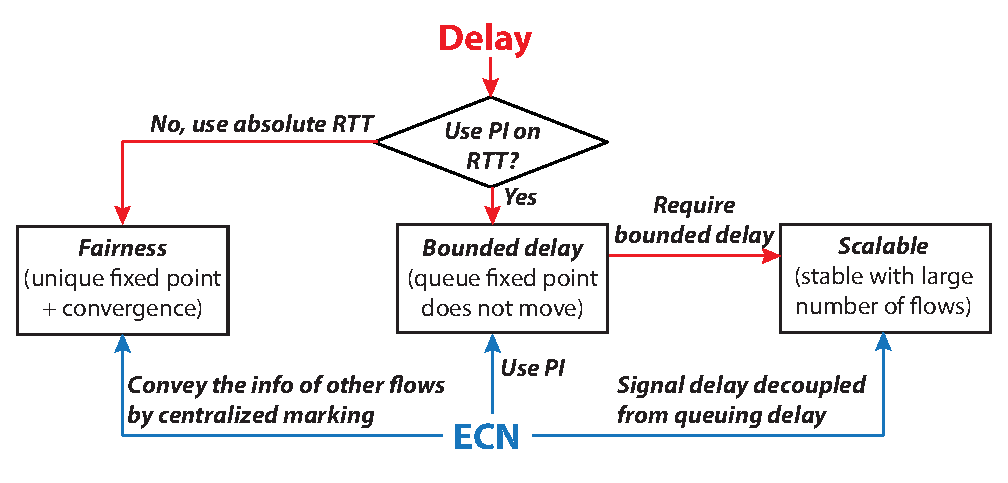
\includegraphics[width=0.45\textwidth]{figures/design_choice.eps}
\vspace{-0.5em}
 \caption{The design choices and desirable properties.}
\vspace{-1.5em}
\label{fig:design_choice}
\end{figure}

% If we are going to
%modify switches to do extra work, numerous other alternatives like
%XCP~\cite{katabi2002congestion}, RCP~\cite{rcp} and pFabric~\cite{pfabric} that
%offer various other tradeoffs must also be considered. We don't dispute this.
%We are actively working on a fuller exploration of PI and other controllers for
%RDMA -- detailed analysis is beyond the scope of this paper.

%%% Local Variables:
%%% mode: latex
%%% TeX-master: "main"
%%% End:
